\documentclass[12pt]{report}
\usepackage[utf8]{inputenc}
\usepackage{graphicx}
\usepackage{float}

\usepackage[left=2cm,right=2cm,top=2cm,bottom=2cm]{geometry}
\usepackage{listings}

\begin{document}
\begin{titlepage}

\newcommand{\HRule}{\rule{\linewidth}{0.5mm}} % Defines a new command for the horizontal lines, change thickness here

\center 
\HRule \\[0.4cm]
{ \huge \bfseries User Guide: \\Representation and relative positioning from visual information}\\[0.4cm]
\HRule \\[1.5cm]

\begin{minipage}{0.4\textwidth}
	\begin{flushleft} \large
		\emph{Realized by:}\\
		\textsc{Asma BRAZI}
	\end{flushleft}
\end{minipage}
~
\begin{minipage}{0.4\textwidth}
	\begin{flushright} \large
		\emph{Proposed by:} \\
		\textsc{Cédric HERPSON}\\
	\end{flushright}
\end{minipage}\\[4cm]


{\large Laboratory of Computer Sciences, Paris 6 \\ Sorbonne University - Faculty of Science and Engineering}\\[3cm] 
{\large August 2019 }\\[3cm] 

\includegraphics[width=0.6\textwidth]{logo.png}\\[1cm] 
\vfill % Fill the rest of the page with whitespace

\end{titlepage}
\tableofcontents
\chapter{Introduction}
This document represents a guide for users. It is necessary to be consulted to ensure a proper configuration of the environment. It is designed to:
\begin{itemize}
    \item Enumerate the different hardware and software prerequisites.
    \item Provide a step-by-step instructions to establish the environment configuration.
    \item Present a brief scenario of how the application runs.
\end{itemize}
\chapter{Getting started}
\paragraph{}
We present in this section the necessary equipment for the use of our application. Also, we specify the essential programs to install.
\section{Hardware prerequisites}
\paragraph{}
The global system can be seen as two independent physical subsystems in interaction. The first one is composed of a computer, and the second one is what we call the autonomous robot. and whose list of components is showed in the figure below.
\begin{figure}[H]
	\begin{center}
		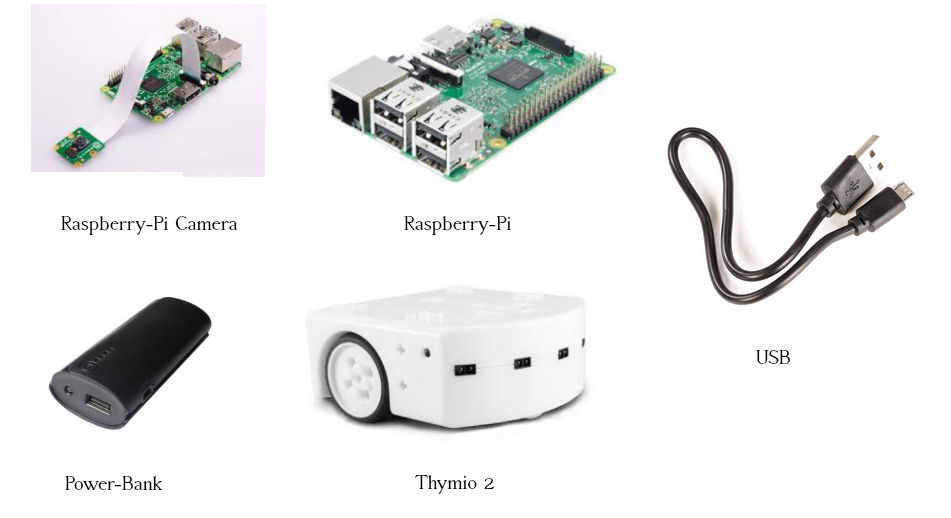
\includegraphics[scale=0.6]{comp.png}
		\caption{The components of the autonomous robot}
	\end{center}
\end{figure}
\paragraph{}
The computer and the autonomous robot are exchanging via Wi-Fi. Nevertheless, the autonomous robot's components are connecting with USB. So, we have to connect the Raspberry-Pi Camera by inserting the cable into the Raspberry-Pi. In the same way, we do so with the Thymio. After that and in order to power the Raspberry-Pi, we use the power-bank which is connected to it with USB. 


\section{OS/Software prerequisites}
\paragraph{}
We need several programs for both subsystems to be able to launch the application. The programs that we have to install on the Raspberry-Pi are:
\begin{itemize}
    \item OpenCV 2.
    \item Python 3.
    \item Asebamedulla.
\end{itemize}
Then, those to install on the computer are:
\begin{itemize}
    \item Java 8.
    \item JMonkey Engine.
    \item Java IDE.
\end{itemize}
\section{Environment configuration}
\paragraph{}
We chose to establish a connection through Wi-Fi rather than Ethernet, because the autonomous robot have to move in its environment. If the environment is large, even a very long Ethernet cable could not be enough.

\subsection{Wireless configuration}
\paragraph{}
As mentioned above, the computer and the Raspberry-Pi must be connected on the same network. In the case of the computer, it is easy to establish the connection, by selecting the name of the desired Wi-Fi network. Nonetheless, connecting the Raspberry-Pi to the network does not seem to be that straightforward.
\paragraph{}
In the case of the Raspberry-Pi, we have to assign an IP address statically to it, so that this IP address is available. In this way, every time the Raspberry-Pi starts, it connects to the router automatically. This is why we opted to fix the IP address. 
\paragraph{}
So, we can assign the IP address of the Raspberry-Pi via SSH, or by connecting it to a screen and a keyboard at least. Once we can manipulate the Raspberry-Pi, we should perform the following steps:
\begin{itemize}
    \item Open a terminal on the Raspberry-Pi.
    \item Execute the command: \emph{sudo nano /etc/wpa\_supplicant/wpa\_supplicant.conf}, in order to modify the file \textbf{wpa\_supplicant.conf}
    \item At the end of the current file, specify the router's id and password as follows: 
    \\\emph{
    network=\\ \{\\
    ssid=network\_id \\
    psk=network\_password \\
    \}}
    \item Save and close the file by typing CTRL-X, then Y.
    \item Load the file to establish the connection with the command: \\ \emph{wpa\_supplicant -iwlan0 -c /etc/wpa\_supplicant.conf \& dhcpcd wlan0}
\end{itemize}
\paragraph{}
At this stage, the Raspberry-Pi is connected to the network. To retrieve its address IP, the command to execute on a terminal is: \emph{hostname -I}
\paragraph{}
After that, we need to set the IP address attributed to the Raspberry-Pi on the file \textbf{config.properties}. We can find this file in the root of the application's directory. Some other attributes may be set like: \textbf{RPi\_id} and \textbf{RPi\_password} (To set the id and the password of the Raspberry-Pi).

\chapter{Launching the application}
\paragraph{}
After having succeeded the configuration, the application is now ready to be launched. Being on a JAVA IDE, the main class to run bears the name of \emph{Principal.java} whose complete path is: \emph{robot-explo/Code/src/explorator/Principal.java} 
\paragraph{}
The launching of the application opens a JME window. In this window, we can see a representation of the environment explored by the autonomous robot in real-time. We show in the figure below an instance of the execution of the application.
\paragraph{}
At the beginning, the application will ask the user to enter the name of the target object from the database. We remind that the target object is the object which the robot will try to find in its environment. 

\paragraph{}
After that, the autonomous robot explores its environment, builds it and try to recognize the target. 

\paragraph{}
Finally, the robot indicates whether it finds the target or not.


\begin{figure}[H]
	\begin{center}
		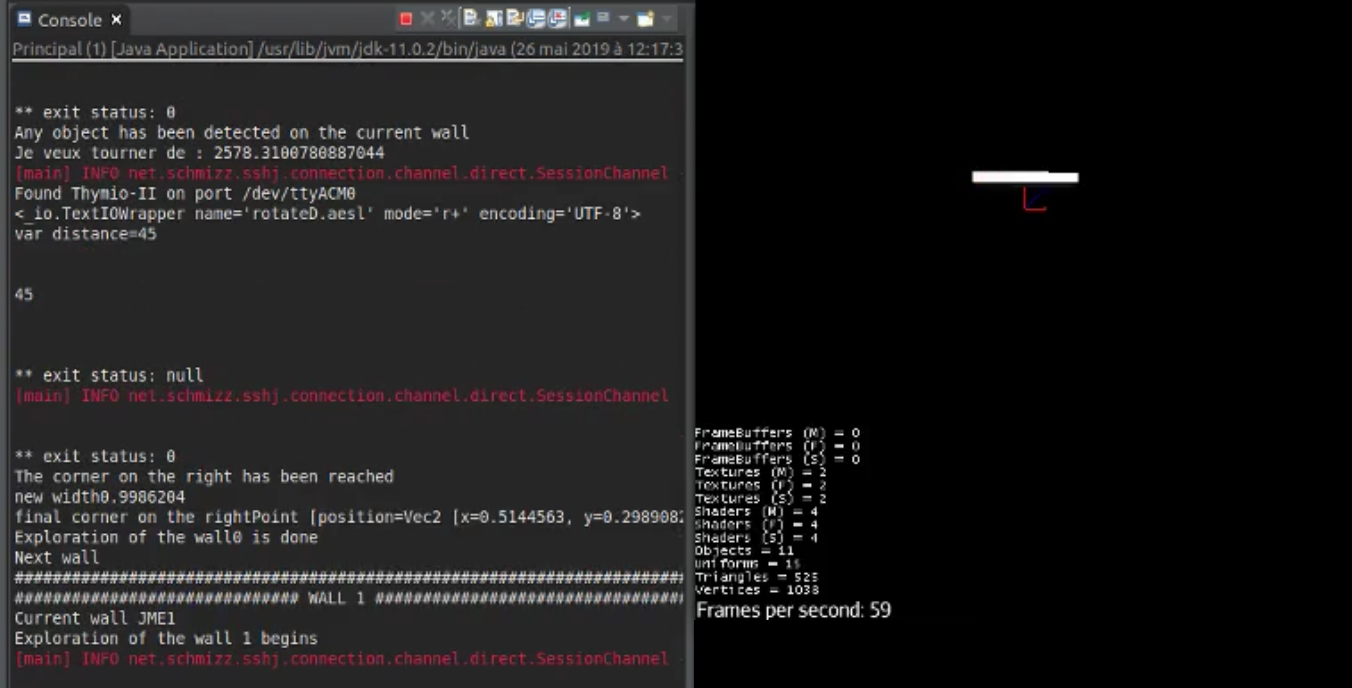
\includegraphics[scale=0.4]{instanceApp.png}
		\caption{An instance of the robot's exploration}
	\end{center}
\end{figure}

\end{document}